\documentclass[12pt]{article}

% Packages
\usepackage[main=slovak,english]{babel}
\usepackage{setspace}
\usepackage{pdfpages}
\usepackage{newtxtext} % Times New Roman
\usepackage[a4paper, left=3.5cm, right=2cm, top=2.5cm, bottom=2.5cm]{geometry} % Mandatory margins
\usepackage{graphicx}
\usepackage[table]{xcolor}
\usepackage{tocbibind}
\usepackage{fancyhdr}
\usepackage{glossaries}
\usepackage{url}
\usepackage{caption}
\usepackage{csquotes}

% Optional packages
%
% Code blocks with syntax highlighting:
\usepackage{listings}
%
% PDF hyperlinks:
%\usepackage{hyperref}

% Thesis metadata
\title{Názov diplomovej práce}
\author{Bc. Alfréd Kôstka}
\def\supervisor{doc. Ing. Severín Hrot, PhD.}
\def\consultant{Mgr. Ignác Šváb} % Optional, remove in titlepage-alt

% University metadata
\def\uid{FI-123456-12345} % Replace with your own student ID
\def\university{PANEURÓPSKA VYSOKÁ ŠKOLA}
\def\faculty{Fakulta Informatiky}
\def\program{Aplikovaná informatika}
\def\fieldofstudy{Informatika}
\def\department{Ústav aplikovanej informatiky}

% Formatting commands
\onehalfspacing % 1.5 line spacing
%
\pagestyle{fancy}
\fancyhead{}
\fancyfoot{}
\fancyfoot[R]{\thepage}
\renewcommand{\headrulewidth}{0pt}%
%
% Bibliography configuration
% style = iso-authoryear, iso-numeric
% use \parencite{} or \textcite{} when using iso-authoryear
% use \cite{} when using iso-numeric
\usepackage[
    style=iso-authoryear,
    ]{biblatex}
\addbibresource{essentials/bibliography.bib}

%
% Acronyms
\makeglossaries
\loadglsentries{essentials/acronyms}
%
% Left align figure/table label
\captionsetup{
    justification=raggedright,
    singlelinecheck=false
}

% Default image options
\setkeys{Gin}{width=0.9\textwidth}  % Set default image width to 90% of text width
\makeatletter
\g@addto@macro\@floatboxreset{\centering}  % Centers all figures by default
\makeatother

% Exclude appendices from adding to list of figures
\newenvironment{appendixfigure}
    {\begin{figure}[h]\renewcommand{\addcontentsline}[3]{}}
    {\end{figure}}

% Code styling
\lstset{
    basicstyle=\ttfamily\small,        % Sets monospace font in small size
    breaklines=true,                   % Enables automatic line breaking for long lines
    backgroundcolor=\color{gray!10},   % Light gray background (10% gray)
    showstringspaces=false,            % Hides visible spaces in strings
    keywordstyle=\color{blue},         % Makes keywords blue
    commentstyle=\color{green!60!black}, % Makes comments dark green
    stringstyle=\color{red},            % Makes strings red
    frame=single,                      % Adds a single frame around the code
    framesep=5pt                      % Space between frame and code
}

% Redefine listing caption name
\renewcommand{\lstlistingname}{Výpis}
\renewcommand{\lstlistlistingname}{Zoznam výpisov}

% Document start
\begin{document}
\selectlanguage{slovak}

% Essentials
\makeatletter
\begin{titlepage}
    \begin{center}
        \MakeUppercase{\textbf{\university}}\\
        \MakeUppercase{\textbf{\faculty}}
    \end{center}
    \textbf{\uid}
    \vspace*{\fill}
    \begin{center}
        \textbf{\large \@title\\}
        \textbf{Diplomová práca}
    \end{center}
    \vspace*{\fill}
    \textbf{\the\year\\\@author}
    
\end{titlepage}
\makeatother
\makeatletter
\begin{titlepage}
    \begin{center}
        \MakeUppercase{\textbf{\university}}\\
        \MakeUppercase{\textbf{\faculty}}
    
    \vspace*{\fill}
    
        \textbf{\large \@title\\}
        Diplomová práca\\
        \textbf{\@author}
    \end{center}
    \vspace*{\fill}
    
    \noindent
    \begin{tabular}{@{}ll@{}}
        Študijný program: & \program \\
        Študijný odbor: & \fieldofstudy \\
        Školiace pracovisko: & \department \\
        Školiteľ: & \professor \\
        Konzultant: & \consultant \\ % Optional
    \end{tabular}
    
    \vspace{2em} 
    \noindent
    \textbf{Bratislava \the\year} 
    
    
    
\end{titlepage}
\makeatother
%
% Replace file with your own:
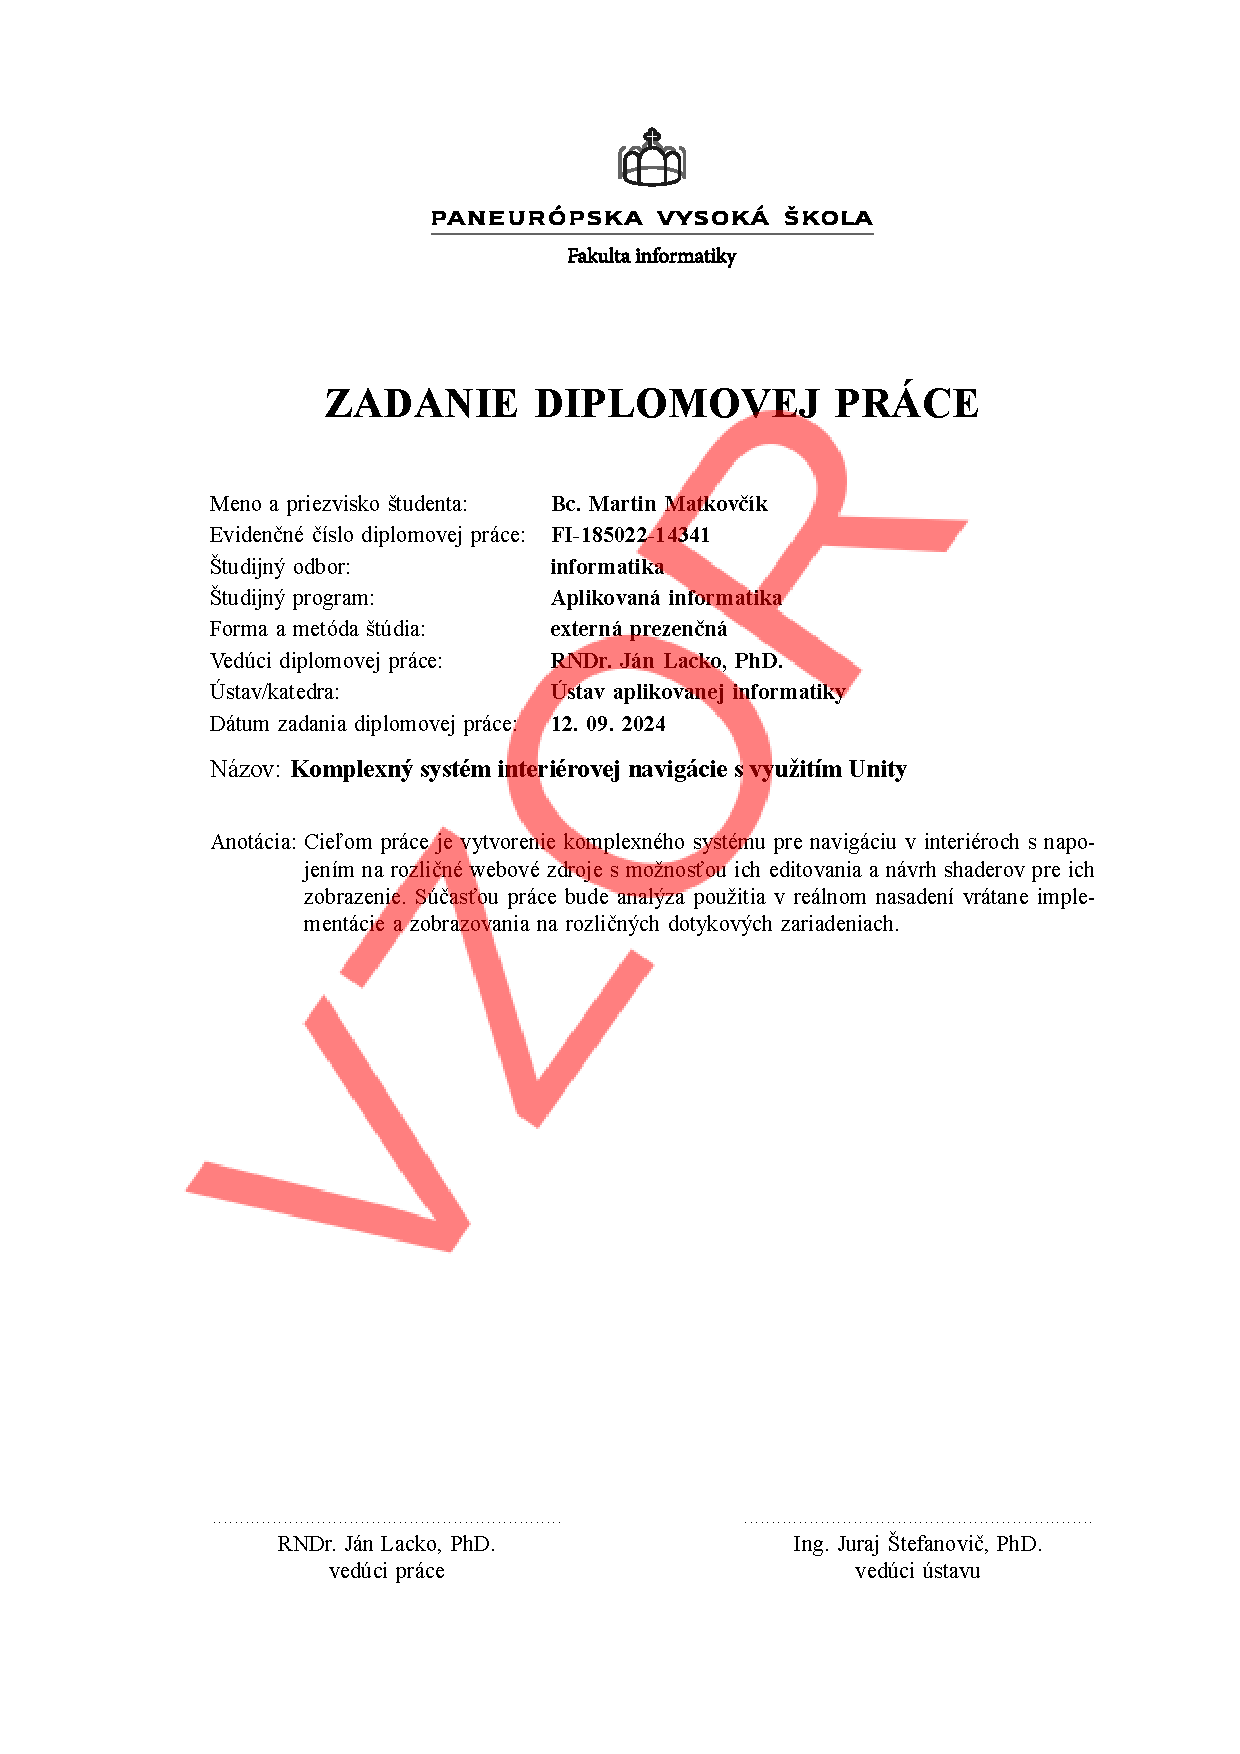
\includepdf{essentials/zadanie.pdf}
%
% Edit:
\begin{flushleft}
    \textbf{Poďakovanie:}\\
    \vspace{1em}
Pri vypracovaní tejto práce by som sa rád poďakoval za odbornú pomoc pánovi \supervisor, ktorý mi poskytol mnoho cenných rád a konzultácií. 
\end{flushleft}


\makeatletter
\vspace*{\fill}
\begin{flushleft}
    \textbf{Čestné prehlásenie:}\\
    \vspace{1em}
    Čestne vyhlasujem, že záverečnú prácu som vypracoval samostatne a že som uviedol všetku použitú literatúru.
\end{flushleft}
\vspace{1em}
\begin{flushright}
    \begin{tabular}{c}
        \makebox[50mm][c]{\dotfill} \\ % Center align the dots
        \makebox[50mm][c]{\@author} % Center align the author name
    \end{tabular}
\end{flushright}
\makeatother

% Redefine the abstract environment to align the title and content to the left
\makeatletter
\renewenvironment{abstract}{
    \if@twocolumn
        \section*{\abstractname}%
    \else
        \normalfont\small
        \begin{flushleft} % Change from center to flushleft
            {\bfseries \abstractname\par}%
        \end{flushleft}%
        \noindent\raggedright
    \fi
}
{
    \if@twocolumn\else\par\fi
}
\makeatother

\begin{abstract}

    Lorem ipsum dolor sit amet, consectetur adipiscing elit. Integer eu lacus leo. Nulla egestas purus non dignissim tincidunt. In sit amet tellus bibendum, lobortis magna ut, sodales mi. Etiam vel eros efficitur purus ultrices vulputate et quis justo. Nunc ultrices tellus a dui mattis, eget laoreet arcu tempor. Donec vestibulum, magna ac fringilla lacinia, libero risus fringilla arcu, nec consectetur nibh justo vel sem. Quisque gravida sit amet elit ut aliquam.\\
    \hfill \break
    Abstrakt obsahuje informáciu o cieľoch práce, jej stručnom obsahu a v závere abstraktu sa charakterizuje splnenie cieľa, výsledky a význam celej práce. Súčasťou abstraktu je 3 - 5 kľúčových slov.
\vspace{1em}\\
\textbf{Kľúčové slová:} Kľúčové slovo 1, Kľúčové slovo 2, Kľúčové slovo 3

\end{abstract}
\pagebreak
\begin{otherlanguage}{english}
\begin{abstract}

    Lorem ipsum dolor sit amet, consectetur adipiscing elit. Integer eu lacus leo. Nulla egestas purus non dignissim tincidunt. In sit amet tellus bibendum, lobortis magna ut, sodales mi. Etiam vel eros efficitur purus ultrices vulputate et quis justo. Nunc ultrices tellus a dui mattis, eget laoreet arcu tempor. Donec vestibulum, magna ac fringilla lacinia, libero risus fringilla arcu, nec consectetur nibh justo vel sem. Quisque gravida sit amet elit ut aliquam.\\ 
    \hfill \break
    Abstrakty v anglickom a slovenskom jazyku sa musia zhodovať.
\vspace{1em}\\
\textbf{Keywords:} Keyword 1, Keyword 2, Keyword 3
\end{abstract}
\end{otherlanguage}

% Content
\tableofcontents
\pagebreak
\listoffigures
\pagebreak

% Glossary
\glsaddall % Add all glossary entries
\printglossary[title={Zoznam skratiek}]
\addcontentsline{toc}{section}{Zoznam skratiek}
\pagebreak

% Chapters:
\section{Úvod}
Lorem ipsum dolor sit amet, consectetur adipiscing elit. Integer eu lacus leo. Nulla egestas purus non dignissim tincidunt. In sit amet tellus bibendum, lobortis magna ut, sodales mi. Etiam vel eros efficitur purus ultrices vulputate et quis justo. Nunc ultrices tellus a dui mattis, eget laoreet arcu tempor. Donec vestibulum, magna ac fringilla lacinia, libero risus fringilla arcu, nec consectetur nibh justo vel sem. Quisque gravida sit amet elit ut aliquam.....
\vspace{1em}
\\V prvej kapitole je popísaný súčasný stav riešenia problematiky. Popísaná je konštrukcia takého systému, ktorý ....
\\V druhej kapitole prezentujeme návrh systému ...
\\V tretej kapitole sme sa zaoberali popisom implementácie systému...

% Examples:
% Define a section
\section{Názov kapitoly}
Lorem ipsum dolor sit amet, consectetur adipiscing elit. Integer eu lacus leo. Nulla egestas purus non dignissim tincidunt. In sit amet tellus bibendum, lobortis magna ut, sodales mi. Etiam vel eros efficitur purus ultrices vulputate et quis justo. Nunc ultrices tellus a dui mattis, eget laoreet arcu tempor. Donec vestibulum, magna ac fringilla lacinia, libero risus fringilla arcu, nec consectetur nibh justo vel sem. Quisque gravida sit amet elit ut aliquam.....

% Define a subsection
\subsection{Názov podkapitoly}
Lorem ipsum dolor sit amet, consectetur adipiscing elit. Integer eu lacus leo. Nulla egestas purus non dignissim tincidunt. 
\begin{itemize}
    \item Položka zoznamu
    \item Položka zoznamu
\end{itemize}
\hfill
\begin{enumerate}
    \item Položka číslovaného zoznamu
    \item Položka číslovaného zoznamu
\end{enumerate}

% Add a figure
\begin{figure}[h]
    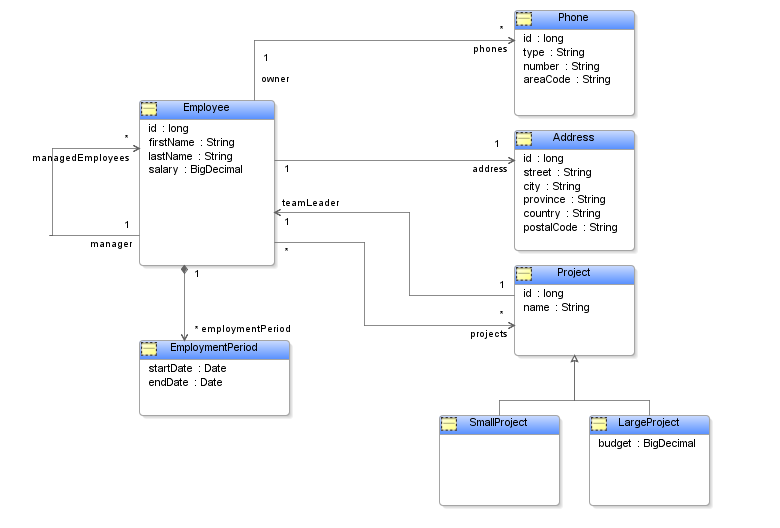
\includegraphics{examples/images/employee-model.png}
    \caption{UML diagram zamestnanca}
    \label{fig:example1}
\end{figure}

% Add citations
\newpage
\noindent
Odkazy na použitú literatúru \parencite{luptak2016thesis} alebo \textcite{borgman2003from}.\footnote{V prípade nejasností alebo pre lepšie pochopenie niektorých pojmov jazyka boli ďalej využívané aj zdroje \parencite{lynch2005where} a \parencite{luptak2016thesis}}
\\Pre citácie používajte normu STN ISO 690, môžete citovať aj v tvare [1], [2],… vtedy v zozname literatúry neuvádzate zdroje abecedne, ale ich uvádzate podľa poradia výskytu v texte. 

% Define a subsubsection
\subsection{Môžete vložiť novú podkapitolu}
\subsubsection{Taktiež aj na úrovni 3}

% Add a table
\begin{table}[!h]
    \centering
    \caption{Názov tabuľky}
    {\color{red} \textbf{Pánsky dres - strih Classic}}\\
    \vspace{1em}
    \rowcolors{2}{white}{gray!30}  
    \begin{tabular}{cccc}  
        \textbf{dres - veľkosť} & \textbf{obvod hrudník} & \textbf{obvod pás (guma)} & \textbf{dĺžka zadného dielu (od krku)} \\
        XS & 96 & 72-80 & 69 \\
        S & 100 & 76-84 & 70 \\
        M & 104 & 80-80 & 71 \\
        L & 108 & 84-96 & 72 \\
        XL & 112 & 88-100 & 73 \\
        XXL & 116 & 92-104 & 75 \\
        XXXL & 120 & 96-108 & 77 \\
    \end{tabular}
    \label{tab:example}
\end{table}

% Add a code block
\begin{lstlisting}[language=Python, caption={Príklad kódu v Pythone}, label={lst:python-example}]    
def hello_world():
    print("Hello, world!")
        
# Example class
class Person:
    def __init__(self, name):
        self.name = name
    
    def greet(self):
        return f"Hello, my name is {self.name}"

# Create instance
person = Person("Alfred")
print(person.greet())
\end{lstlisting} 

\section{Záver}
Nezabudnite na Záver a zhodnotenie.\\  
Cieľ bakalárskej práce bol splnený.

% Bibliography
\newpage
\printbibliography[title={Použitá literatúra}]
\addcontentsline{toc}{section}{Použitá literatúra}

% Appendices
\section*{Prílohy}
\addcontentsline{toc}{section}{Prílohy}
\begin{enumerate}
    \item Relationship Metamodel: Štruktúra metamodelu (www.example.com)
    \begin{appendixfigure}
        \centering
        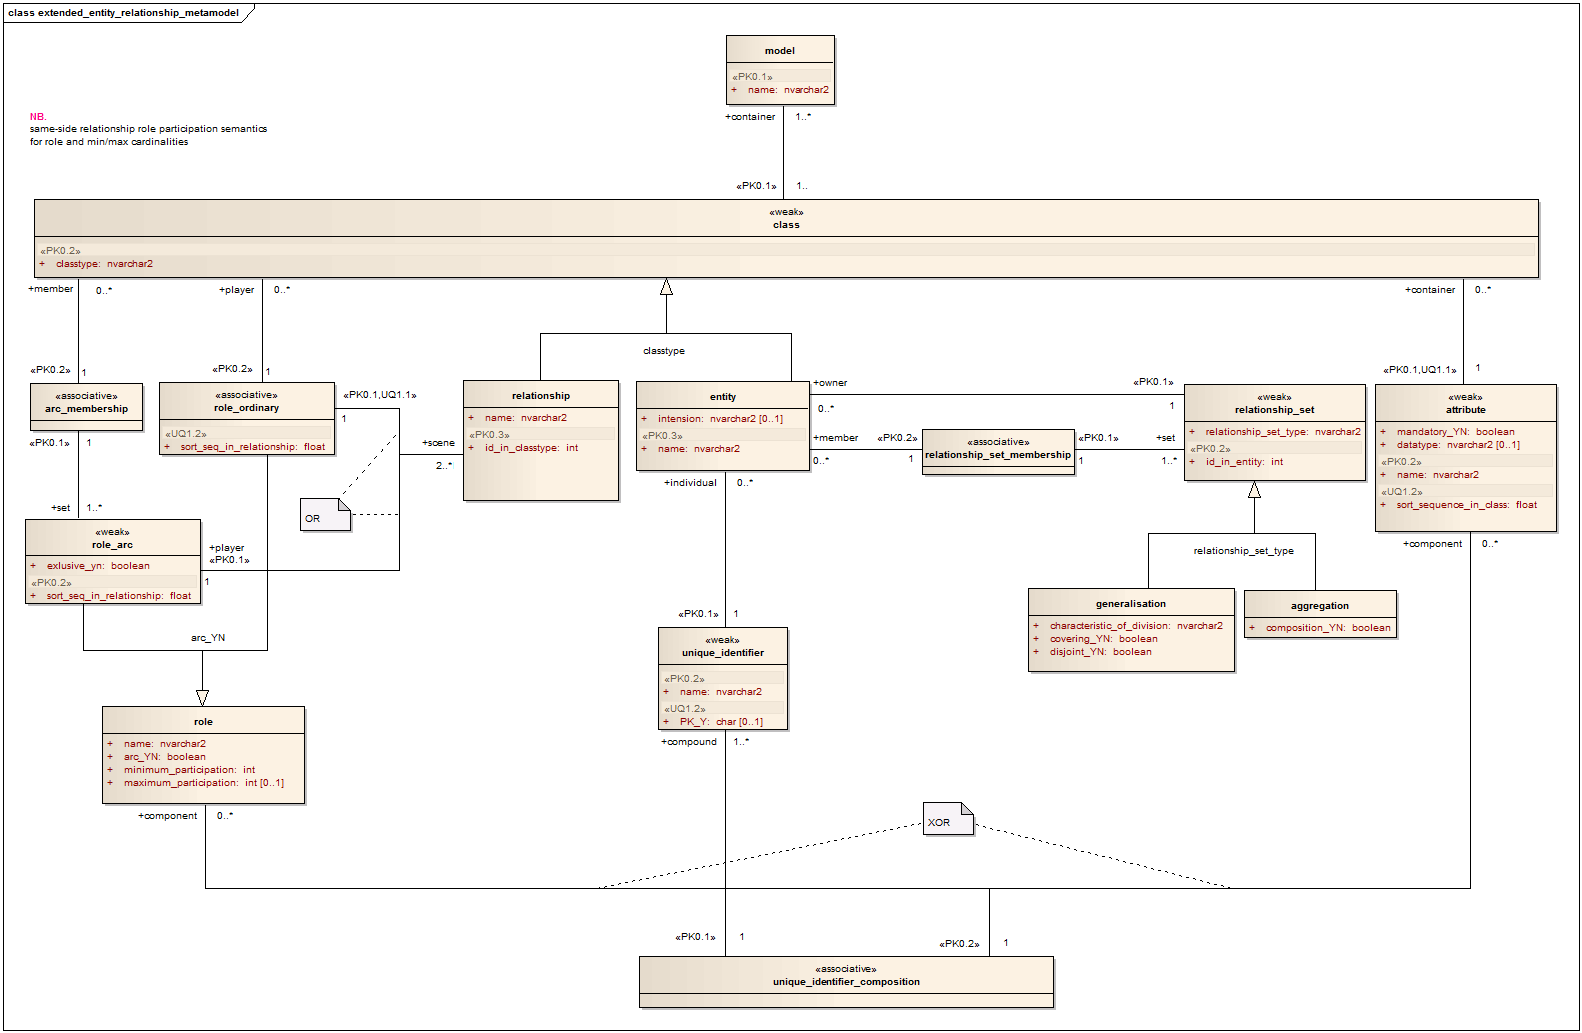
\includegraphics[height=0.75\textwidth,angle=90]{examples/images/metamodel.png}
        \caption{Popis obrázku}
        \label{fig:appendix-image1}
    \end{appendixfigure}
\end{enumerate}

\end{document}